\documentclass{article}

\pagenumbering{gobble}

\usepackage{graphicx}
\usepackage[square,numbers]{natbib}
\renewcommand{\bibname}{References}
\usepackage{xcolor}
\usepackage{enumitem}
\usepackage{bigfoot}
\usepackage{pdfpages}
\usepackage{hyperref}
\hypersetup{
    colorlinks,
    linkcolor={black},
    citecolor={blue!35!black},
    urlcolor={blue!35!black}
}

\usepackage[bottom]{footmisc}
\usepackage[nottoc]{tocbibind}
\usepackage{amsmath}
\usepackage[utf8x]{inputenc}
\usepackage{amssymb, upgreek}
\usepackage[toc,page]{appendix}

\usepackage{color}
\definecolor{keywordcolor}{rgb}{0.7, 0.1, 0.1}   % red
\definecolor{commentcolor}{rgb}{0.4, 0.4, 0.4}   % grey
\definecolor{symbolcolor}{rgb}{0.0, 0.1, 0.6}    % blue
\definecolor{sortcolor}{rgb}{0.1, 0.5, 0.1}      % green
\definecolor{errorcolor}{rgb}{1, 0, 0}           % bright red
\definecolor{stringcolor}{rgb}{0.5, 0.3, 0.2}    % brown

\usepackage{listings}
\def\lstlanguagefiles{lstlean}
\lstset{language=lean}

\begin{document}

\section*{Defense: Provable Determinism in Reactors}

\begin{center}
    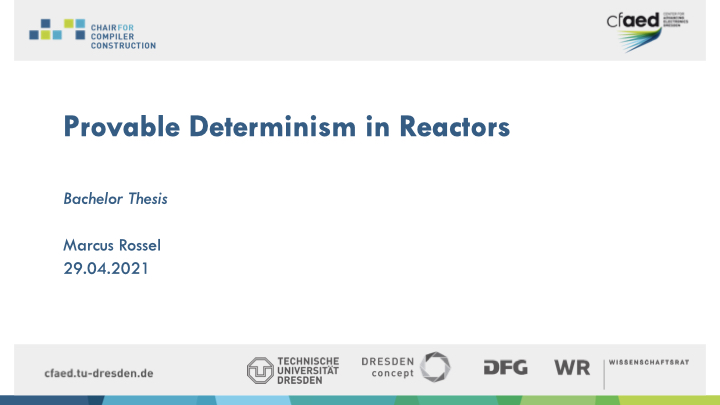
\includegraphics[width=\columnwidth]{Slides/Slide 1.jpeg}
\end{center}

I'd like to start off this talk with a short story.

\begin{center}
    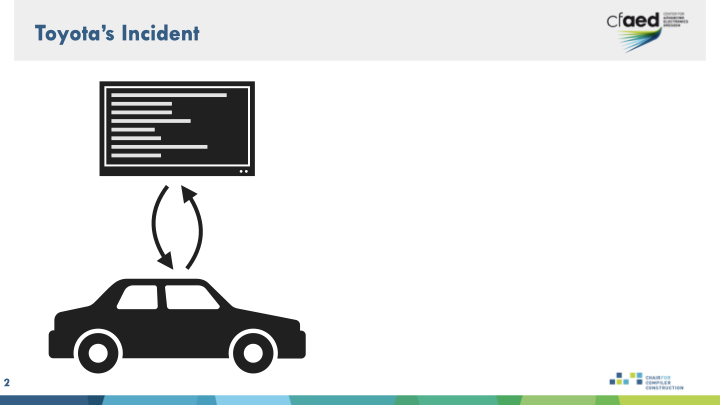
\includegraphics[width=\columnwidth]{Slides/Slide 2.jpeg}
\end{center}

I'm not sure if you might have heard of it, but around the year 2010, the car manufacturer Toyota recalled millions of vehicles due to several cases of ``unintended acceleration'' --- acceleration of vehicles, not intended by the driver.
Notably, Toyota experienced a 400\% increase of these unintended accelerations after having started to use new \emph{electronic} throttles in certain models.
That is, while traditional gas pedals were connected \emph{mechanically} to the accelerator, these new ones involved indirection through a software system.
Such software systems are usually called ``cyber-physical'' systems, as they interact with the physical world.

\begin{center}
    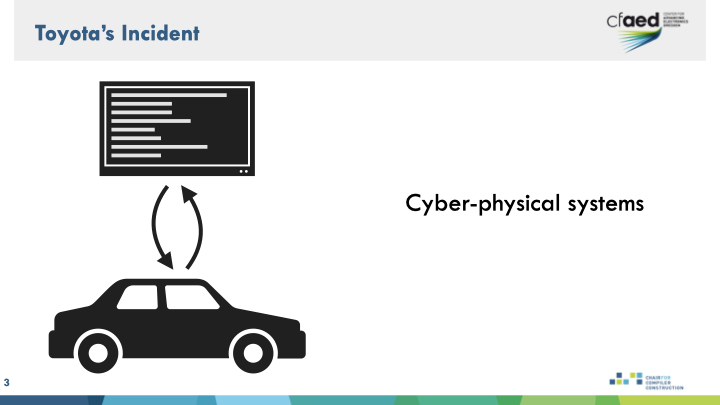
\includegraphics[width=\columnwidth]{Slides/Slide 3.jpeg}
\end{center}

During the recalls around 2010, the source of this issue was investigated, in part by NASA.
Of course, one target of the investigation was the software system responsible for acceleration.
In their report, NASA concluded that the software could not be found to be the culprit.
But that came with a big caveat:
They also found the software to be hard to test, therefore making it impossible to rule it out as the source of the problem.
And that's a conclusion from \emph{NASA}, the people who've managed to write software with less than 1 error per 10.000 lines of code.
What this goes to show, is that cyber-physical systems need to be testable!

\begin{center}
    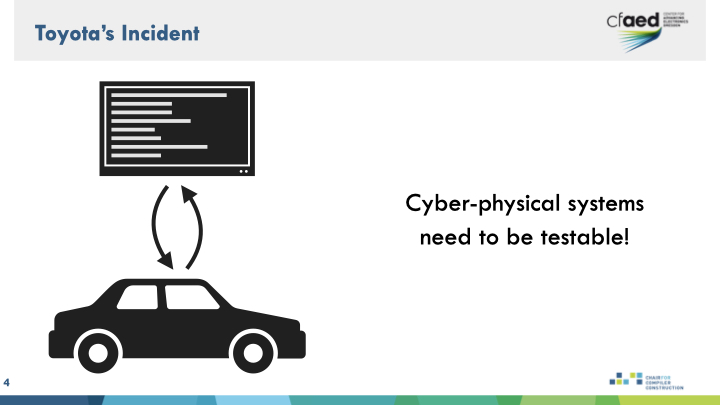
\includegraphics[width=\columnwidth]{Slides/Slide 4.jpeg}
\end{center}

First of all, because if they aren't, then we can't be sure that our system behaves correctly.
And secondly, because correct behavior is especially important for cyber-physical systems, as consequences of failure can be dire.

The first protagonist in this talk intends to help us with this.
It's a model for writing concurrent testable code --- especially in the context of cyber-physical systems --- called the Reactor model.
And the name of our protagonist actually tells us something about it.
It's called the Reactor \emph{model}, because it is a mathematical model.

\begin{center}
    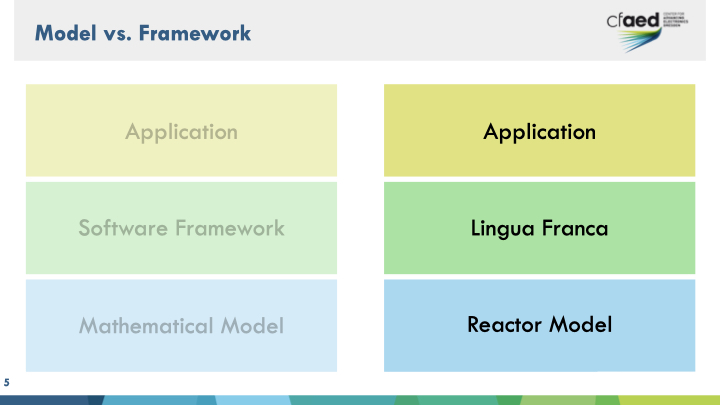
\includegraphics[width=\columnwidth]{Slides/Slide 5.jpeg}
\end{center}

If we consider its place in the context of software, we can see that this is not the same things as a framework, but rather a mathematical foundation for which we build frameworks.
In the context of the Reactor model, the corresponding software framework is called \emph{Lingua Franca}.
But we're going to ignore that here, and focus on the mathematical model of reactors.

\begin{center}
    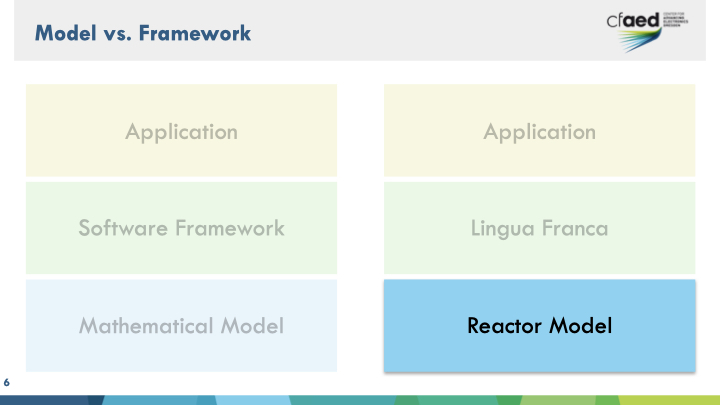
\includegraphics[width=\columnwidth]{Slides/Slide 6.jpeg}
\end{center}

Seeing that there already exists a software implementation, we might ask why we even need a mathematical model.
The reason is really the same as for most use cases of mathematics, which is that we want to be \emph{very} certain about certain things.
In \emph{this} context, the things we want to be certain about are properties of our software, like the satisfaction of timing constraints or \emph{determinism}.
And the way to be really certain about something is of course to \emph{prove} it, for which we need ... mathematics. 
Hence, we have the Reactor model which allows us to obtain mathematical certainty about certain properties of our software.
Now, there are some meta issues that are part of this setup.
For example, how can we be sure that Lingua Franca actually adheres to the Reactor model? 
And for that matter, how can we even be sure that our model is mathematically correct?
Well, this brings us to the second protagonist of this talk: Lean Theorem Prover.

\begin{center}
    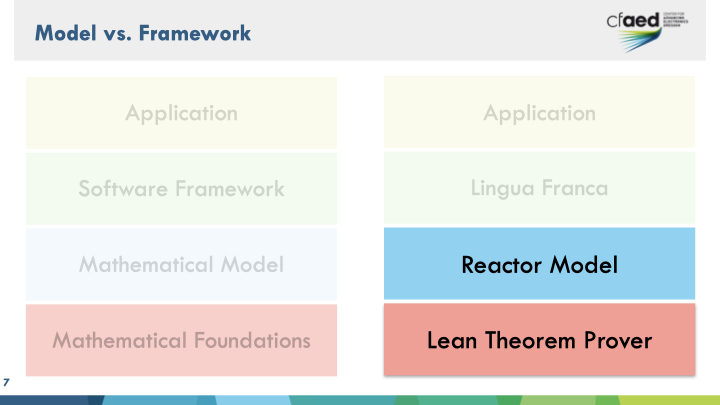
\includegraphics[width=\columnwidth]{Slides/Slide 7.jpeg}
\end{center}

Lean will be the mathematical foundation for our model, as well as a tool that will provide us with certainty about its correctness.
So in next 15 minutes, you'll learn about a model for writing testable concurrent code, as well as a tool for formalizing and verifying mathematics.  

Let's start with our first protagonist: the Reactor model.

\begin{center}
    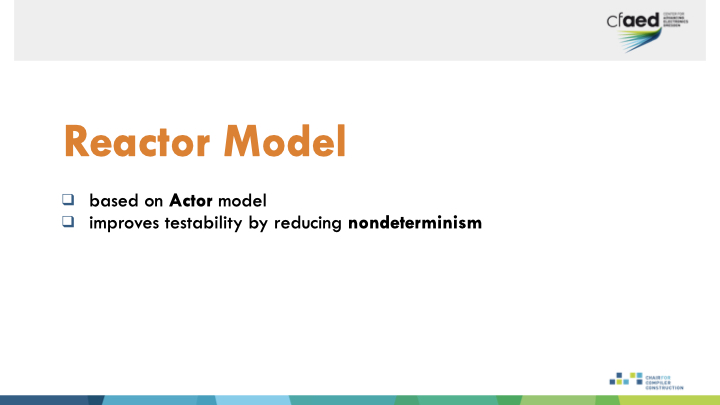
\includegraphics[width=\columnwidth]{Slides/Slide 8.jpeg}
\end{center}

The promise was that reactors will allow us to write testable concurrent code.
And here's how.
Firstly, it's based on the Actor model, which will help us with concurrency.
But more importantly (for this talk at least), it improves testability by reducing nondeterminism (which is otherwise present in actors).
To understand both of these aspects, let's look at an example.

\begin{center}
    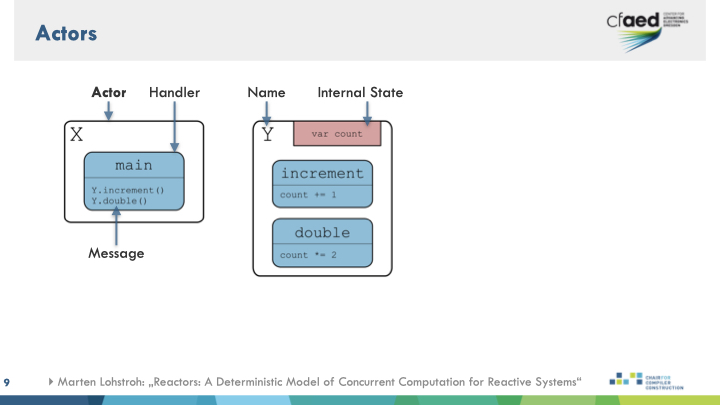
\includegraphics[width=\columnwidth]{Slides/Slide 9.jpeg}
\end{center}

What you can see here is a network of actors.
Actors are these isolated units of functionality.
As the actor \verb|Y| shows, they can contain internal \emph{state}.
This state is accessible to an actor's \emph{handlers}.
Handlers are kind of like methods on an object.
The way in which actors communicate with each other is by \emph{messages}.
For example, in actor \verb|X| the \verb|main| handler sends the messages \verb|increment| and \verb|double| to \verb|Y|.
When \verb|Y| receives these messages, it will execute the corresponding handlers.
This model gives a very simple model for concurrent execution:
Each actor runs concurrently (on an own thread).
And even though this setup is concurrent, it executes deterministically.
To demonstrate what I mean by that, consider what would happen if we started execution with the \verb|main| handler.

\begin{center}
    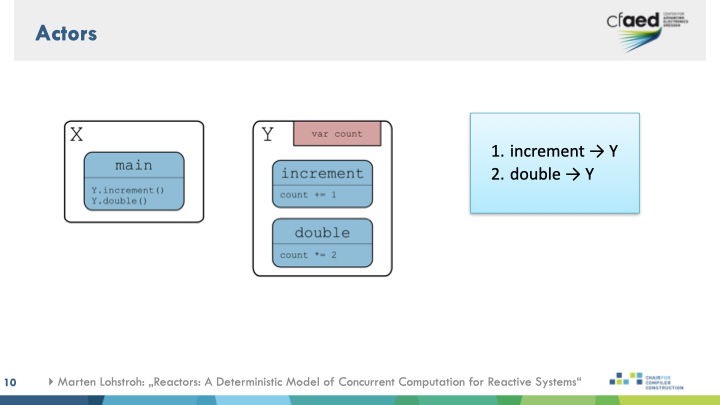
\includegraphics[width=\columnwidth]{Slides/Slide 10.jpeg}
\end{center}

First the \verb|increment| message is sent to \verb|Y| and then the \verb|double| message is sent to \verb|Y|.
Hence, this system is deterministic: there's only one result that can come out of calling \verb|main|.
But now consider a slight modification to this example:

\begin{center}
    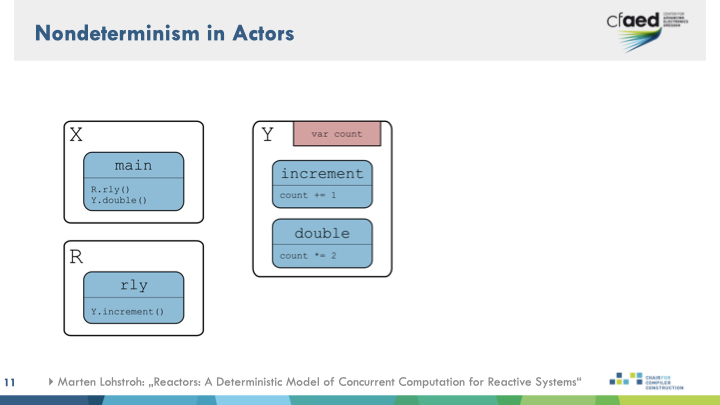
\includegraphics[width=\columnwidth]{Slides/Slide 11.jpeg}
\end{center}

What we've done here is relay the \verb|increment| message sent by \verb|X.main| through some other actor \verb|R|.
So instead of sending \verb|Y.increment| directly from \verb|X.main|, we instead send \verb|R.rly| and then \verb|R|'s \verb|rly| handler sends \verb|Y.increment| for us.
This doesn't change anything, right?
Well, actually it introduces nondeterminism into our system.
Consider what happens now when we start execution on \verb|main|.

\begin{center}
    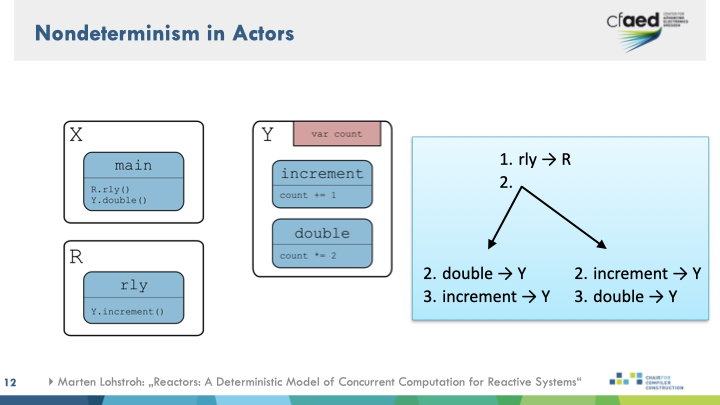
\includegraphics[width=\columnwidth]{Slides/Slide 12.jpeg}
\end{center}

First the \verb|rly| message is sent to \verb|R| and \verb|double| message is sent to \verb|Y|.
Then \verb|R| sends the \verb|increment| message to \verb|Y| as a result of its \verb|rly| handler.
But does that mean that this message arrives at \verb|Y| before or after the \verb|double| message?
There's no right answer here --- we'll just have to see which message arrives first.
This is an example of nondeterminism: 
Calling \verb|X.main| can lead to different results for the new state of \verb|Y|. 
As you can imagine, this makes the system basically untestable.
Writing a test case for this scenario will sometimes fail and sometimes succeed, so we're none the wiser.
And that's exactly why the Reactor model aims at reducing nondeterminism.
Let's consider briefly, how reactors could be used to solve this problem.

\begin{center}
    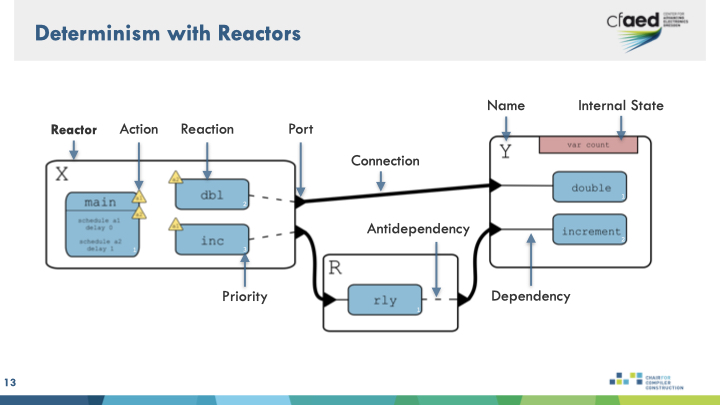
\includegraphics[width=\columnwidth]{Slides/Slide 13.jpeg}
\end{center}

The point of this slide is not for you to understand exactly what is going on here, but rather to draw connections between actors and reactors.
First of all, as you can see, the Reactor model is a bit more complex than the Actor model.
It still defines these isolated units, now called \emph{reactors}.
And reactors still contain internal state, as well as the analog of handlers, now called \emph{reactions}.
But as you can see, there are now these explicit connections between the reactors, via certain interface points called \emph{ports}.
So when a reaction wants to trigger some reaction in another reactor, it has to be explicitly connected to it via these ports.

\begin{center}
    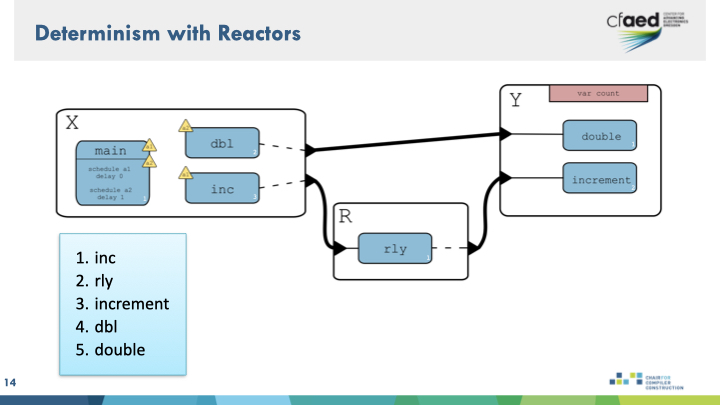
\includegraphics[width=\columnwidth]{Slides/Slide 14.jpeg}
\end{center}

An important result of this kind of setup is that, if we execute this system, there's only one possible order in which reactions can be executed.
Hence, this system is deterministic.
And in turn, testing this system would actually be possible.
But only because \emph{this} system is deterministic, does that mean that all systems of reactors are deterministic?

To answer this question we need to formalize reactors as well as a notion of computation on them.
And as previously mentioned, we'll do this using a tool called Lean.

\begin{center}
    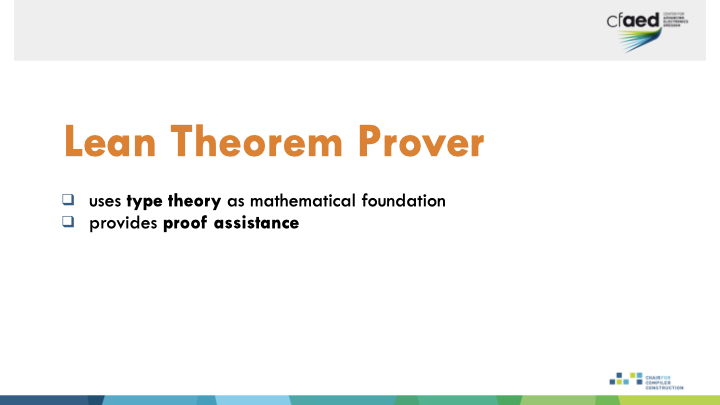
\includegraphics[width=\columnwidth]{Slides/Slide 15.jpeg}
\end{center}

There are two important things you need to know about Lean.
First, it's based on type theory. 
And second, it provides proof assistance.
Let's first consider what it means for Lean to be based on type theory.

\begin{center}
    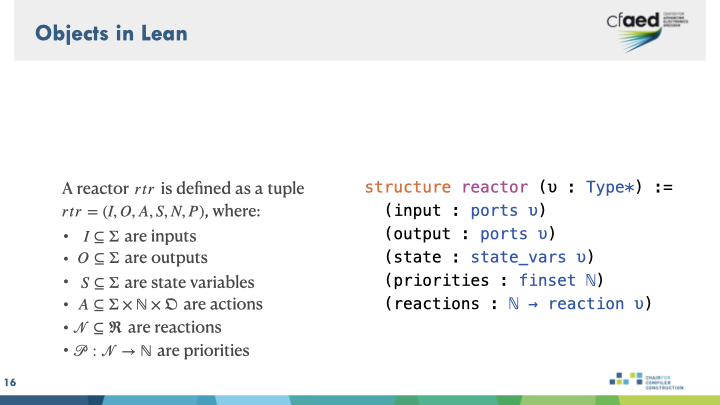
\includegraphics[width=\columnwidth]{Slides/Slide 16.jpeg}
\end{center}

In normal mathematics, you might be used to definitions like the one shown on the left.
Here we define what a reactor is, by describing its components, which are in turn subsets of other sets.
The definition shown on the right also defines reactors, but in Lean.
And even though this looks a lot like computer code, remember, this is a mathematical definition.
Although, there is one aspect from programming languages that carries over:
Each field in this structure is assigned a \emph{type}.
And the thing were defining --- reactors --- is in fact also a type.

\begin{center}
    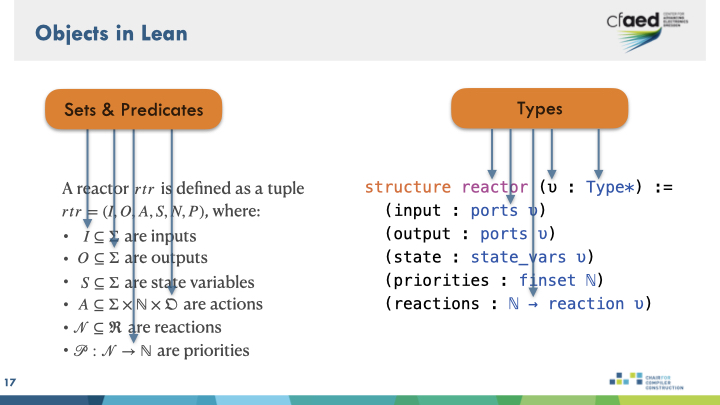
\includegraphics[width=\columnwidth]{Slides/Slide 17.jpeg}
\end{center}

So when we say that Lean is based on type theory, that means it's not based on the standard set theory.
Hence, in Lean the idiom is not ``everything is a set'', but rather ``everything is a typed term''.

Some of you will know that set theory isn't actually the lowest layer in standard mathematics --- it builds on predicate logic.
So if we use types instead of sets, then what is our underlying logic?
There is none.
Instead, we build our logic system using types.

\begin{center}
    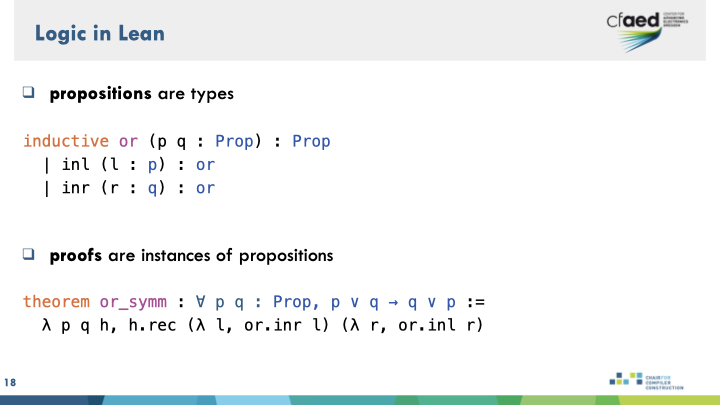
\includegraphics[width=\columnwidth]{Slides/Slide 18.jpeg}
\end{center}

If we take a brief look at how this is done, we will also get a strong understanding of how we can rigorously prove things using Lean.
The way propositions are represented in type theory is as types.
For example, we can define the $\vee$-connective as a type.
Of course, a connective isn't really useful if we're not connecting anything.
Hence, the \verb|or| type depends on two other propositions \verb|p| and \verb|q|.
You can think of these (kind of) as generic type parameters.
Since types should ideally be constructable, we provide constructors for the \verb|or|-type as well. 
But that really begs the question:
What does it mean to construct an instance of a proposition?
That's precisely the next point of this slide.
Instances of propositions are proofs for them.
So if we, for example, wanted to prove that $\vee$ is symmetrical, we could do that by constructing an instance of the type \verb|∀ p q : Prop, p ∨ q → q ∨ p|.
The last line on this slide shows a term for constructing such an instance.
And while this \emph{is} a proper proof of the symmetry of $\vee$, it's really not easy to understand this proof as a human.
Optimally, we would like to prove theorems in a more linear and human-friendly way.
This brings us to Leans second role: it's a proof assistant.
To show what this means, let's prove the symmetry of $\vee$ using a nicer method called tactic mode.

\begin{center}
    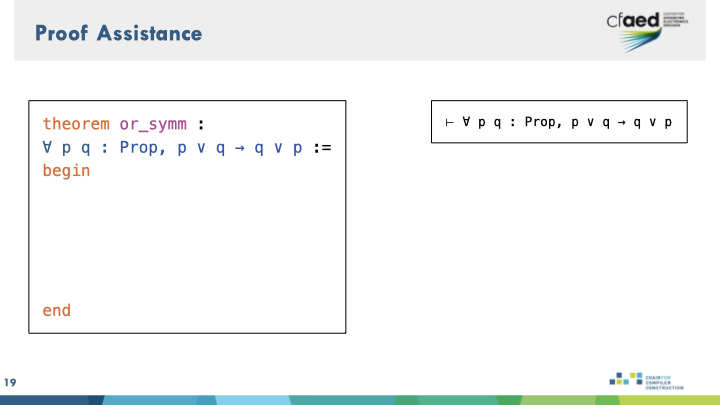
\includegraphics[width=\columnwidth]{Slides/Slide 19.jpeg}
\end{center}

On the left is where we're going to prove our theorem, and on the right is what is called the \emph{goal state}.
When we prove a theorem using tactic mode, Lean will help us by providing us with information about the state of our proof.
One piece of information is the remaining subgoal, i.e. the remaining proposition(s) that need(s) to be proven to complete the proof of the theorem.
Currently, our remaining subgoal is precisely the theorem we're trying to prove --- which makes sense, given that we haven't started the proof yet.
Now, in tactic mode we prove theorems linearly: as sequences of steps.
For example, if we want to prove a $\forall$, we can do this in the ``traditional math'' way:
We choose an arbitrary but fixed element of the set (or in this case \emph{type}) over which we are quantifying, and show that the theorem holds for that arbitrary element.
This is done by using the \verb|intros| tactic.

\begin{center}
    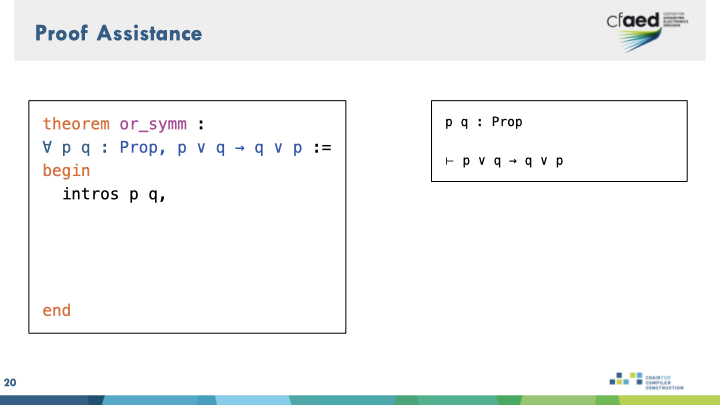
\includegraphics[width=\columnwidth]{Slides/Slide 20.jpeg}
\end{center}

Since the $\forall$ quantified over two variables, we're introducing two instances.
We call them \verb|p| and \verb|q|.
As you can see, applying this tactic changes our goal state.
First of all, at the top we can now see our current \emph{assumptions}.
Here our assumptions are that we have some instances \verb|p| and \verb|q| of type \verb|Prop|.
Also, our remaining subgoal has changed, such that the $\forall$ has been eliminated.
So let's keep going.
In the next step we use the standard practice for proving an implication:
We assume its premise to be true, and prove that the consequence must then also hold.
We can again use the \verb|intro| tactic for this.

\begin{center}
    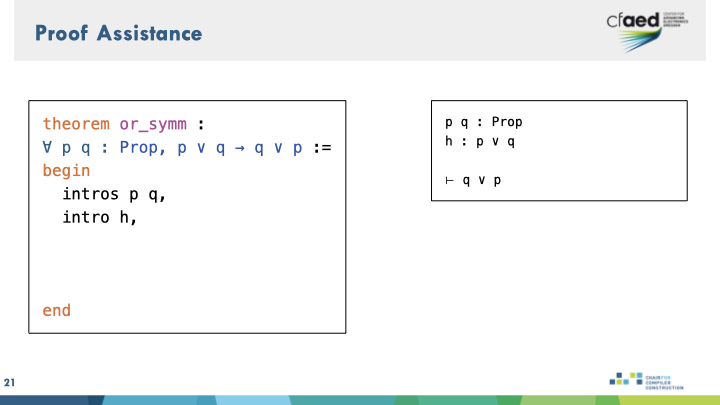
\includegraphics[width=\columnwidth]{Slides/Slide 21.jpeg}
\end{center}

Again our goal state changes.
We now have a new assumption \verb|h|, which is a proof of \verb|p ∨ q|.
All that's left to do is to use that assumption somehow, to prove \verb|q ∨ p|.
One way of approaching this, is by performing a proof by cases on \verb|h|.
In the first case we assume that the reason why \verb|h| is true is that its left side holds.
In the second case we assume that the reason why \verb|h| is true is that its right side holds. 

\begin{center}
    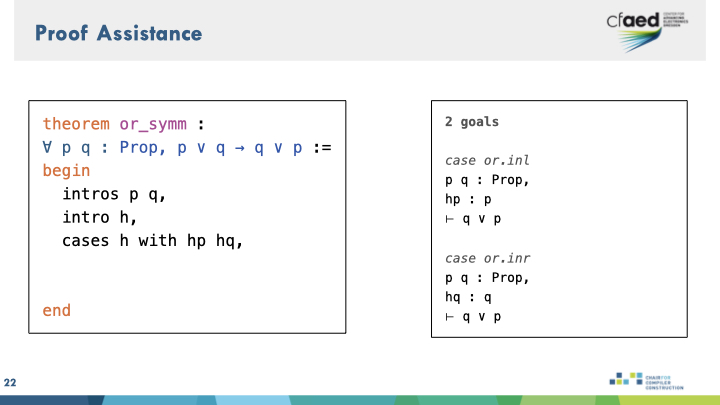
\includegraphics[width=\columnwidth]{Slides/Slide 22.jpeg}
\end{center}

Since we now need to show that the theorem we're trying to prove really holds in both cases, we have two subgoals.
Each of these subgoals can be proven by directly calling one of the constructors of the \verb|or| type we've seen before.

\begin{center}
    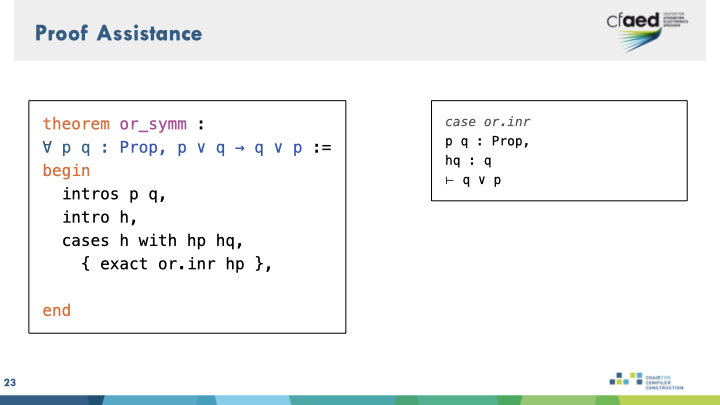
\includegraphics[width=\columnwidth]{Slides/Slide 23.jpeg}
\end{center}

And once we've done that for both cases, our theorem has been proven.

\begin{center}
    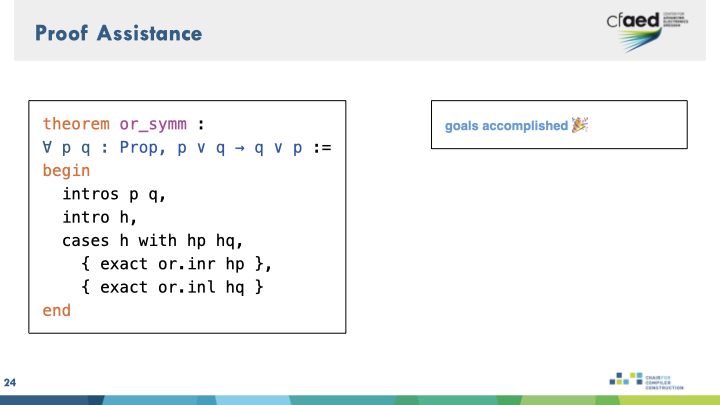
\includegraphics[width=\columnwidth]{Slides/Slide 24.jpeg}
\end{center}

So once we see this ``goals accomplished'', we know that our proof is complete and more importantly that it is correct.
No human reviewer needs to check that our proof is valid --- Lean does that for us.

% 16:30

I hope you now have at least some intuition for what the Reactor model is, and what Lean is.
In the next and last chapter of this talk we can now consider what I wrote about in my thesis on \emph{Provable Determinism in Reactors}.

\begin{center}
    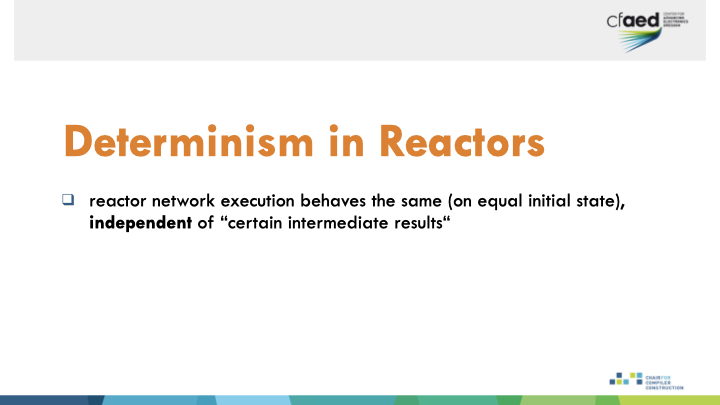
\includegraphics[width=\columnwidth]{Slides/Slide 25.jpeg}
\end{center}

That is, in the thesis we prove (using Lean) that a simple version of the Reactor model is deterministic, \emph{independent} of ``certain intermediate results''.
If you understand what this means, you've basically understood my thesis --- so let's dive into it.

\begin{center}
    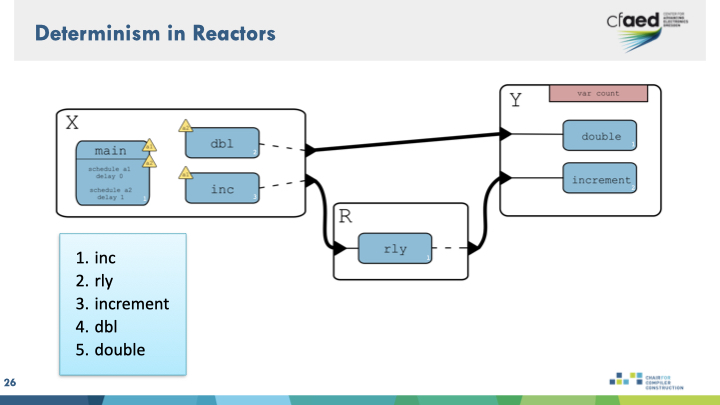
\includegraphics[width=\columnwidth]{Slides/Slide 26.jpeg}
\end{center}

First, let's reconsider a previous slide.
When we talked about how the Reactor model makes computation deterministic, I said that this was the case, because the Reactor model forces our system into only being able to resolve the order of reactions in exactly one way.
This isn't actually \emph{quite} true.
Instead, it \emph{is} possible to have ambiguity about the order of some reactions, but only when the order of those reactions doesn't affect the outcome of computation.
You can think of this kind of like the order of operations in arithmetic.

\begin{center}
    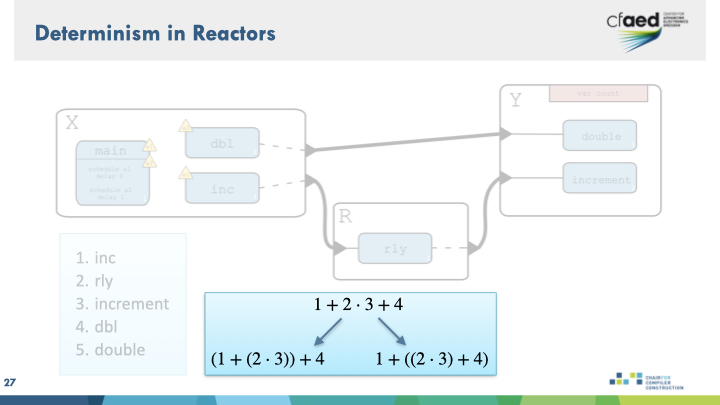
\includegraphics[width=\columnwidth]{Slides/Slide 27.jpeg}
\end{center}

There are multiple ways in which we can execute the operators, as long as multiplication comes before addition.
That is, multiplication takes \emph{precedence} over addition --- and as long as we heed this precedence, we will get the same result from the computation of the formula.

In a reactor network the precedences between reactions aren't as trivially determined.
They are a result of how reactors' ports are interconnected, how reactions connect to those ports and certain priorities assigned to reactions within a reactor.
So the first step in executing a reactor network is always to create a graph that captures these precedence relations.

\begin{center}
    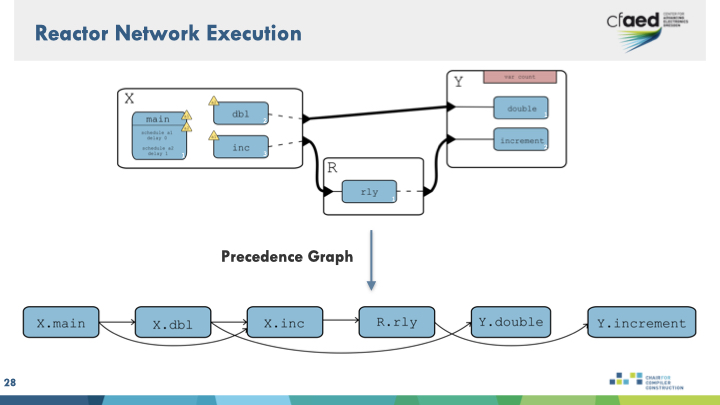
\includegraphics[width=\columnwidth]{Slides/Slide 28.jpeg}
\end{center}

To actually get a \emph{concrete} order of reactions that heeds the precedences, we create a topological ordering over this graph.

\begin{center}
    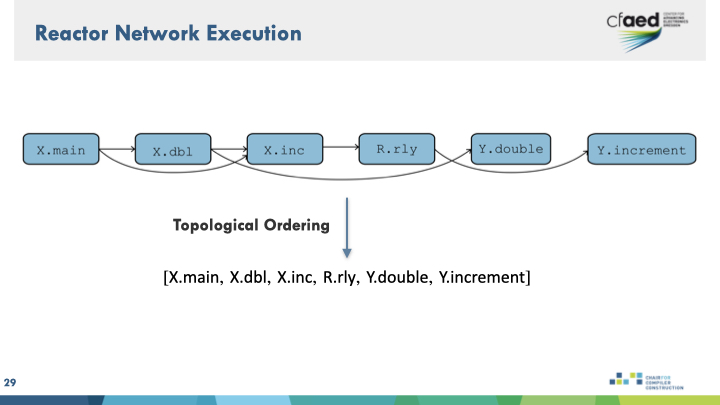
\includegraphics[width=\columnwidth]{Slides/Slide 29.jpeg}
\end{center}

This list of reactions then represents the order in which they are executed.

But here arises the crux of determinism:
A single reactor network may have multiple precedence graphs, and more importantly, a precedence graph may have multiple topological orderings over it.
So how do we know, that they all produce the same result upon execution?
Or going back to our arithmetic example... 

\begin{center}
    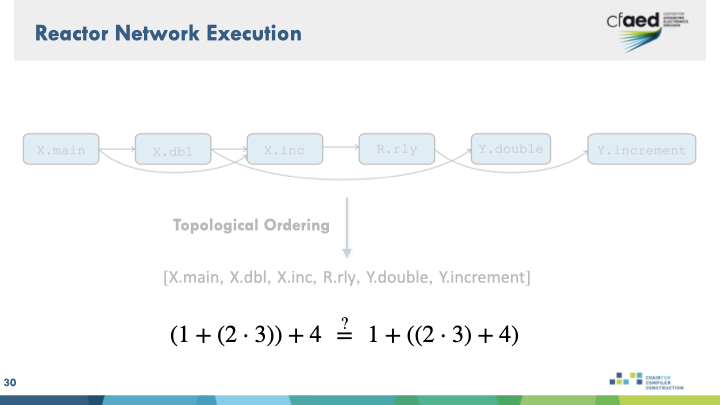
\includegraphics[width=\columnwidth]{Slides/Slide 30.jpeg}
\end{center}

How do we know that both orders of execution produce the same result?
We prove it.
And that precisely what I've done in my bachelor thesis.

\begin{center}
    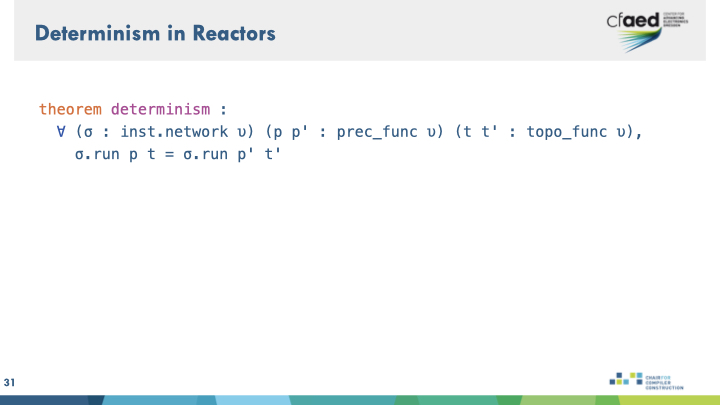
\includegraphics[width=\columnwidth]{Slides/Slide 31.jpeg}
\end{center}

So, \verb|determinism| is a theorem, just like the symmetry of $\vee$ was.
But now the proposition we're proving is of course something different.
Let's dissect it real quick.
We say that, if \lstinline|σ| is some reactor network...

\begin{center}
    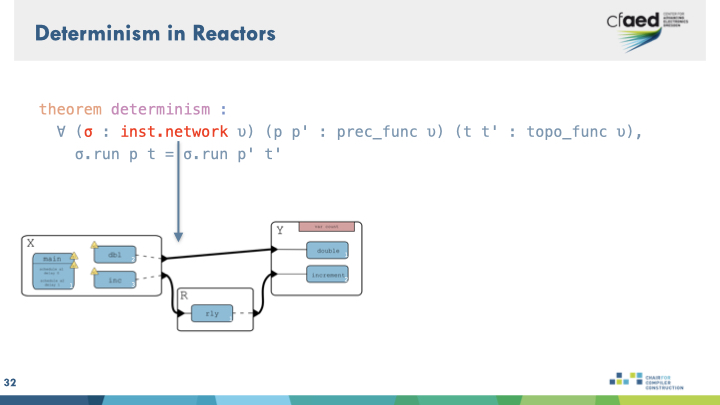
\includegraphics[width=\columnwidth]{Slides/Slide 32.jpeg}
\end{center}

... then executing (i.e. ``running'') that network produces the same result ...

\begin{center}
    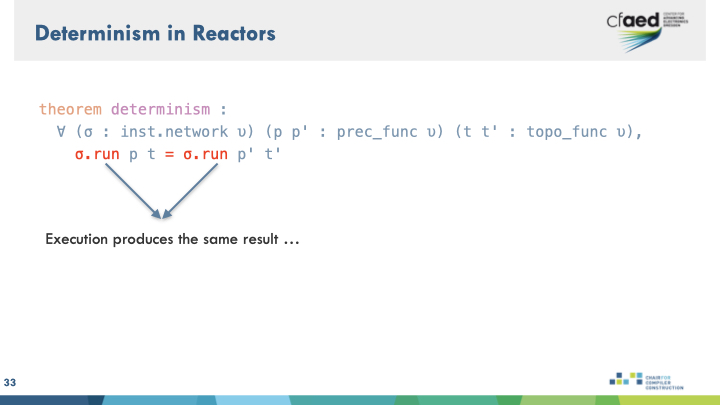
\includegraphics[width=\columnwidth]{Slides/Slide 33.jpeg}
\end{center}

... independent of the parameters \verb|p/p'| and \verb|t/t'|.

\begin{center}
    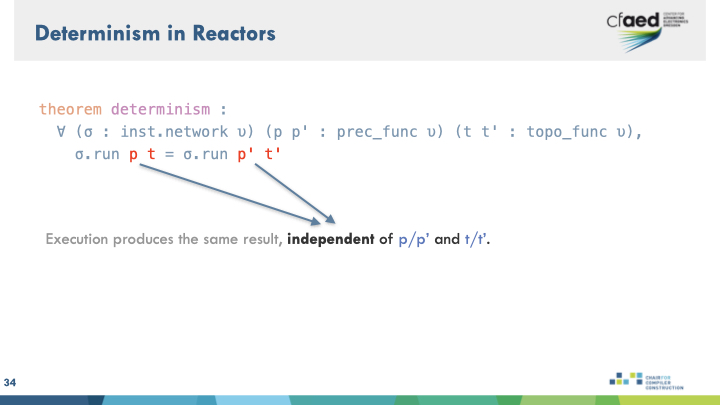
\includegraphics[width=\columnwidth]{Slides/Slide 34.jpeg}
\end{center}

And those parameters are precisely what specifies the precendence graph and topological ordering.

\begin{center}
    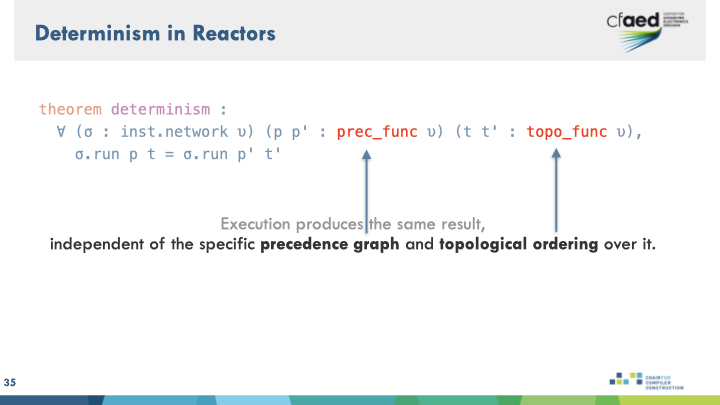
\includegraphics[width=\columnwidth]{Slides/Slide 35.jpeg}
\end{center}

So in total, we've proven that reactor network execution produces the same result, independent of the specific order in which reactions are executed, as long as they adhere to precedence constraints.
Or in other words, reactors are deterministic. 

\begin{center}
    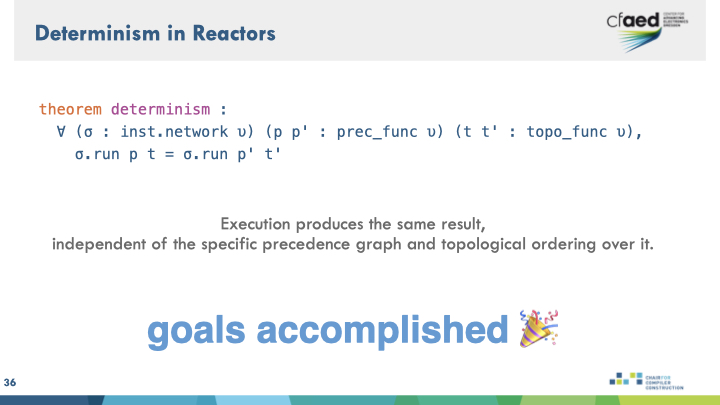
\includegraphics[width=\columnwidth]{Slides/Slide 36.jpeg}
\end{center}

\end{document}
